\documentclass{amia}
\usepackage{graphicx}
\usepackage[labelfont=bf]{caption}
\usepackage[superscript,nomove]{cite}
\usepackage{color}
\usepackage{multirow}
\renewcommand*{\thefootnote}{\fnsymbol{footnote}}

\begin{document}

\title{Machine Learning Methods for Discourse Segmentation of Communications in E-Mail Based Behavioral Interventions}

\author{Mehedi Hasan, BS$^{1}$\footnote[1]{Authors provided equal contribution. \label{footnote1}}, Alexander Kotov, PhD$^{1}$\textsuperscript{\ref{footnote1}}, Sylvie Naar, PhD$^{2}$, Gwen L. Alexander, PhD$^{3}$, April Idalski Carcone, PhD$^{4}$}

\institutes{
$^1$Department of Computer Science, Wayne State University, Detroit, Michigan \\  
$^2$Center for Translational Behavioral Research, Department of Behavioral Sciences and Social Medicine, Florida State University, Tallahassee, Florida\\
$^3$Department of Public Health Sciences, Henry Ford Health System, Detroit, Michigan\\
$^4$Department of Family Medicine and Public Health Sciences, School of Medicine, Wayne State University, Detroit, Michigan\\
}

\maketitle

\noindent{\bf Abstract}
\textit{Communication science approaches to developing effective behavior interventions, such as motivational interviewing (MI), are limited by traditionally manual qualitative coding of communication exchanges, which is a very resource-intensive and time-consuming process. This study focuses on the analysis of e-Coaching sessions, behavior interventions that are delivered via email and grounded in the principles of MI. A critical step towards automated annotation of e-Coaching communication exchanges is segmentation of emails into textual fragments that correspond to MI behaviors. In this work, we formulate this task as a classification problem and propose lexical, punctuation and topic features to address it. We experimented both with traditional machine learning methods, such as Support Vector Machine, Naive Bayes and K-Nearest Neighbor (KNN) classifiers and recurrent neural networks (RNNs). Experimental results indicate that KNN outperformed RNNs achieving 0.986 macro F1-score overall, and 0.779 and 0.993 macro F1-score for detecting ``new segment'' and ``same segment'' classes, respectively.}

\section*{Introduction}
The emergence of e-Health technologies opened up new ways to deliver a variety of behavioral interventions to any demographic group of patients in any geographical location. Motivational interviewing (MI), an evidence-based communication technique to increase intrinsic motivation and self-efficacy for behavior change\cite{miller2012motivational,miller2009ten,miller2009toward}, is one type of these interventions. MI sessions are generally aimed at eliciting ``change talk'', or statements of intrinsic motivation about patients' own desire, ability, reasons, need for and commitment to behavior change, which have been established by previous research\cite{apodaca2009mechanisms} as a reliable mediator of health behavior change. However, communication science approaches to understanding the efficacy of MI are inherently limited by traditional qualitative coding methods. 

Qualitative coding of motivational interviews with pre-defined codes has been traditionally performed manually by trained annotators, which is a tedious and resource-intensive process that involves several iterations of reading, comprehension and interpretation of interview transcripts. Rapidly developing computational technologies, specifically, machine learning methods, offer a unique opportunity to accelerate this process. In particular, machine learning methods have been successfully applied to a variety of analytical tasks involving textual data, such as classification\cite{nigam2000text} and sentiment analysis\cite{wang2012baselines}. In our previous work, we examined the utility of machine learning methods for automated annotation \cite{hasan2016study,kotov2015interpretable} and analysis \cite{hasan2018predicting} of in-person MI sessions. Specifically, we demonstrated that machine learning methods can be utilized for annotation of MI transcripts according to a simple communication code scheme with the accuracy comparable to human coders\cite{hasan2016study}. Experimental data utilized in these studies, however, were prepared by transcribing audio conversations, which were clearly segmented into utterances by a counselor, a patient, and, in some cases, a caregiver. 

In this study, we focus on the analysis of e-Coaching sessions, behavior interventions that are delivered via email and grounded in the principles of motivational interviewing. Specifically, the e-Coaches involved in this study used emails to communicate motivation-enhancing messages that encourage healthy eating among GenY adolescents. e-Coaching data is comprised of email responses, which are free-text documents, unlike more traditional dyadic clinical interviews that are naturally segmented into utterances due to their conversational nature.

The unstructured nature of e-Coaching exchanges poses a unique set of challenges for their qualitative analysis. A significant barrier to fully automating the behavior coding process of e-Coaching emails is their segmentation into textual fragments that correspond to distinct communication behaviors. Automating this task is a unique and challenging problem due to the following major reasons:

\begin{enumerate}
\item Emails are unstructured text that contains informal information exchange in a non-traditional format.
\item Discourse segments in e-Coaching emails do not necessarily correspond to sentences or collection of sentences. One sentence can be segmented into multiple MI behavior fragments. On the other hand, an MI behavior may comprise several sentences.
\end{enumerate}

Figure~\ref{fig:text-segment} illustrates a segmentation of an e-Coaching email exchange, in which the first sentence is segmented into 2 MI behavior fragments, while the fourth and fifth segments correspond to one and three sentences, respectively. Segmentation of e-Coaching emails corresponds to a special type of discourse analysis \cite{webber2012discourse} aimed at better understanding the effective e-Coaching communication strategies and revealing the unique socio-psychological characteristics of a patient.

\begin{figure}[!htb]
    \centering
    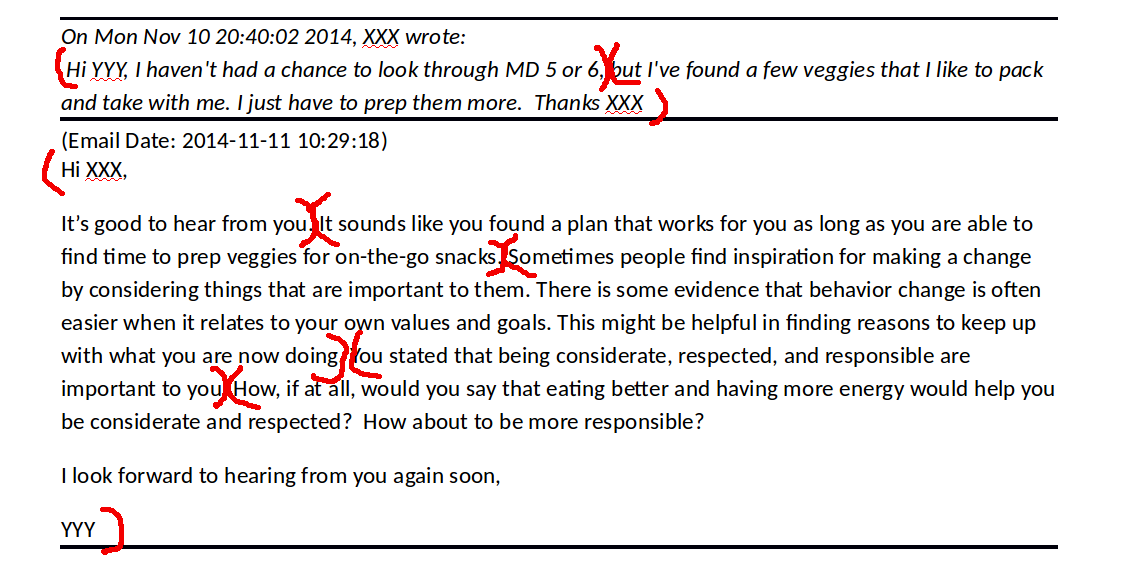
\includegraphics[width=0.9\textwidth]{figures/segment-example.png}
    \caption{\textbf{Example of e-Coaching emails segmented into fragments that correspond to MI behaviors of an e-Coach and a patient}.}
    \label{fig:text-segment}
\end{figure}

The goal of this research study is to assess the applicability of machine learning methods for automated segmentation of e-Coaching emails into textual fragments corresponding to individual behaviors, which is the first step of the coding process of e-Coaching communications. In particular, we introduced lexical, topic and punctuation features and experimented with both traditional supervised machine learning methods, such as Support Vector Machine (SVM), Naive Bayes (NB) and K-Nearest Neighbor (KNN) classifiers, and deep learning methods, such as Long Short Term Memory (LSTM) and Gated Recurrent Unit (GRU), to find the best performing method and feature combination. 

Relevant previous work in the biomedical domain primarily focused on segmentation of text into sections and headers\cite{apostolova2009automatic,denny2009evaluation,tepper2012statistical,cho2002text} or sentence boundary detection\cite{griffis2016quantitative,kreuzthaler2015detection,treviso2016sentence}. Apostolova et al.\cite{apostolova2009automatic} applied SVM along with word-vector cosine similarity metric combined with several heuristics to segment clinical reports into sections, such as demographics, history, procedure, finding and impression. After identification of each line in the document, Tepper et al. \cite{tepper2012statistical} trained Maximum Entropy models for section classification. Denny et al.\cite{denny2009evaluation} proposed a SecTag algorithm, which combined natural language processing techniques, terminology-based rules, and Naive Bayes classifier to identify the sections and headers that achieved 99\% recall with 95.6\% precision. On the other hand, SVM based on prosodic and part of speech features \cite{kreuzthaler2015detection} and recurrent convolutional neural networks using word embeddings \cite{griffis2016quantitative} were utilized for detecting sentence boundaries. Segmentation of e-Coaching emails is different from traditional shallow discourse analysis of conversations \cite{galley2003discourse} in that the focus is on segmentation, rather than on determining the types of transitions between the utterances or assigning utterances to speakers.

Recently, an online clinical intervention called MENU GenY \cite{alexander2017motivations} (Making Effective Nutrition Choices for Generation Y) was proposed and evaluated. MENU GenY is a technology-based public health intervention that relies on personalized e-coaching to encourage increased fruit and vegetable intake among young adults, aged 21-30. The goal of MENU GenY was to develop a better coding dictionary among GenY to improve eating habits. However, segmentation of clinical conversation in the context of electronically delivered interventions, in particular, segmentation of clinical interaction text into groups of MI behaviors, is still performed manually, which slows down qualitative analysis of these interventions. This study introduces a novel computational approach to address this problem and the authors are unaware of any other work that focused on the same problem.  

\section*{Methods}
\subsection*{\textit{Data collection}}
The experimental dataset for this work was constructed from 49 e-coaching sessions, which include a total of 3,138 segmented and annotated MI behaviors. Each session represents an MI intervention delivered via email. During pre-processing, we removed all non-ASCII characters and applied stemming to normalize morphological variants of related concepts, such as ``eating'', ``eats'', and ``eat''. We formulate the segmentation task as a binary classification problem, as illustrated in Figure~\ref{fig:classifier} and experimented both with traditional machine learning methods, such as Support Vector Machine (SVM), Naive Bayes (NB) and K-Nearest Neighbor (KNN) classifiers and recurrent neural networks (RNNs), such as Long Short Term Memory (LSTM) and Gated Recurrent Unit (GRU). For NB, SVM and KNN models, e-Coaching email exchanges are partitioned into adjacent word pairs. Each pair is classified into either ``new segment'' or ``same segment'' class. The gold standard is manually segmented where adjacent word pairs are classified into ``new segment'' class. If all adjacent word pairs of a block of text are classified into ``same segment'' class, the entire block is treated as one textual fragment corresponding to a single MI behavior. In total, we obtained 95,421 word pairs, which include 3,138 ``new segment'' and 92,283 ``same segment'' instances. For RNNs, a block of text was taken as input sequence, such that one-hot encodings of each word or punctuation marks in a block were used as input into an RNN and binary labels (1 or 0) corresponding to ``new segment'' and ``same segment'' classification decision were considered as the output of RNN at each step. In the gold standard, words within the same segment were assigned the label of 0 and the last word or punctuation mark of a segment were assigned the label of 1.    

\begin{figure}[!htb]
    \centering
    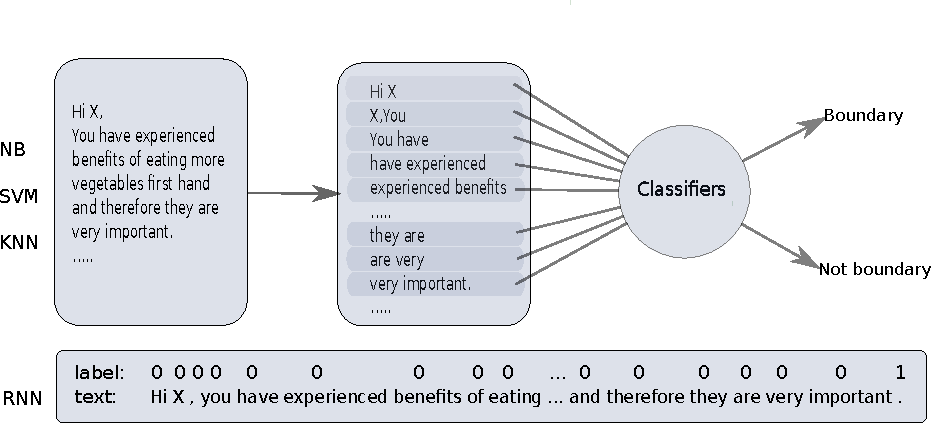
\includegraphics[width=0.80\textwidth]{figures/classifier.pdf}
    \caption{\textbf{Transformation of text segmentation task into text classification task}.}
    \label{fig:classifier}
\end{figure}

\subsection*{\textit{Features}}

We utilized three types of features in conjunction with SVM, NB and KNN methods: lexical, punctuation and topic features. Lexical features represent each word in a pair as a binary vector, in which 1 corresponds to the word in question and 0 to all other words. Since topic models\cite{kotov2015interpretable,hashimoto2016topic,lu2016modeling} have been shown to be effective semantic abstractions of individual words, we derived topic features from Labeled LDA\cite{ramage2009labeled}, a topic model for annotated corpora. We considered each textual segment in the training set as a document and the MI code assigned to the segment as a label. First, we derived a label-specific multinomial $p(w|l)$ for each label $l$ from the word distributions $p(w|l,z)$ for topic $z$ specific to label $l$ by marginalizing over topics: 

$$p(w|l) = {\sum_{z=1}^{K}{p(w|z,l)}}$$

where $K$ is the optimal number of topics experimentally determined to minimize perplexity. After that, distributions over labels, $p(l|w)$, for each word were obtained from label-specific multinomials $p(w|l)$ using Bayesian inversion: 

$$p(l|w) = \frac{p(w|l)p(l)}{p(w)}$$

where $p(l)$ is the prior probabilities of label $l$ in the training set and $p(w)$ is the prior probability of word $w$ in the language model estimated from the training set using maximum likelihood. We use the distribution $p(c|w)$ as the topical feature vector, which shows how indicative each word $w$ is for a particular behavior code $l$. Topical features allow to abstract away from individual words and detect segment boundaries by indirectly capturing transitions between behavior codes when only observing a pair of words that are specific to different behavior codes. Punctuation marks, which correspond to one of the symbols \{`.', `,', `!', `?', `:', `;', `-'\} between a pair of words, are also employed as a feature, since punctuation marks designate the boundary of a sentence, clause, and phrase and often also correspond to segment boundary.   

\subsection*{\textit{Classifiers}}

We experimented both with traditional classifiers, including Naive Bayes (NB)\cite{pedregosa2011scikit}, Support Vector Machine (SVM)\cite{chang2011libsvm}, K-Nearest Neighbor (KNN)\cite{pedregosa2011scikit} and two variants of Recurrent Neural Networks (RNNs)\cite{bengio1993problem}: Long Short Term Memory (LSTM)\cite{hochreiter1997long} and Gated Recurrent Unit (GRU)\cite{cho2014properties}. 

\textbf{Naive Bayes}: this model estimates the prior probability of classes along with conditional probabilities of each feature given the class. Then, the posterior probability is computed to predict the class for each sample by applying the Bayes rule with the assumption that features are conditionally independent. We used Multinomial Naive Bayes in experiments.

\textbf{Support Vector Machine}: state-of-the-art supervised classification method proven to be effective for text categorization\cite{joachims1998text} for its ability to cope with high dimensional input feature space. SVM finds the hyperplane that maximizes the separation between the closest ``new segment'' and ``same segment'' training examples. We used SVM with polynomial kernel in experiments.   

\textbf{K-Nearest Neighbor}: this method considers each training sample as a point in the input feature space. For a new test sample, Euclidean distance is calculated to find the k-nearest classified neighbors from the training set. Finally, the test sample is classified into a majority class of its k-nearest neighbors. We experimentally determined that best performance was achieved when the number of neighbors is 3. 

\textbf{Recurrent Neural Networks}: RNN is a neural network architecture designed to capture sequential patterns. When we predict the ``new segment'' point using RNNs, particular combinations of words in a sequence will indicate the change of MI behavior. Long Short Term Memory (LSTM) networks\cite{hochreiter1997long} are a special type of RNN that are capable of handling variable size input sequence and have an internal memory that can be reset. GRU\cite{cho2014properties} is a variant of LSTM mathematically represented by the following formula:

\begin{equation}
z_t = \sigma(W_zx_t + U_zh_{t-1} + b_z)
\label{eq:firstgru}
\end{equation}
\begin{equation}
r_t = \sigma(W_rx_t + U_rh_{t-1} + b_r)
\label{eq:resetgru}
\end{equation}
\begin{equation}
\tilde h_t = tanh(W_hx_t + r_t \odot U_hh_{t-1} + b_h) 
\label{eq:candidategru}
\end{equation}
\begin{equation}
h_t = z_t \odot h_{t-1} + (1-z_t) \odot \tilde h_t
\label{eq:lastgru}
\end{equation}  
In Eq.~\ref{eq:firstgru}-\ref{eq:lastgru}, $\sigma$ corresponds to sigmoid function and $\odot$ designates an element-wise product. The update gate $z_t$ and reset gate $r_t$ at time step $t$ are computed by the Eq.~(\ref{eq:firstgru}) and~(\ref{eq:resetgru}), where $W_z$, $W_r$, $W_h$, $U_z$, $U_r$, $U_h$ are the weight matrices and $b_z$, $b_h$ and $b_r$ are bias vectors. The activation $h_t$ of the GRU at time $t$ is a linear combination of previous activation $h_{t-1}$ and the candidate activation $\tilde h_t$, which is represented by Eq.~(\ref{eq:lastgru}) and~(\ref{eq:candidategru}). Our GRU model includes one hidden layer, output layer, and input layer. We reset our model state after feeding each input sequence where input was given as one-hot encoding of word vector. Since LSTM and GRU use one-hot vector as input, results for these models are reported only when lexical and punctuation features are used. We experimentally determined that the best performance is achieved when the number of hidden units is 25, batch size is 1, and Adam is used for optimization.         
  
\subsection*{\textit{Evaluation metrics}}
We report standard metrics for experiments (precision, recall, and F1-measure) to evaluate the performance of binary classifiers\cite{aas1999text}. However, accuracy is not reported as a performance metric because accuracy is highly sensitive to the prior class probabilities and does not fully describe the actual difficulty of the decision problem for an unbalanced dataset. The results are reported based on 5 folds cross-validation and weighted macro-averaging over the folds. We also estimate the area under the receiving operating characteristics (ROC) curve\cite{kumar2011receiver} (AUC) metric due to its effectiveness in measuring the quality of binary classifiers for imbalanced datasets \cite{hu2015kernelized}. 

\section*{Results}
Experimental results are evaluated with ``boundary'' and ``not boundary'' classes as well as their weighted average, which are shown in Table~\ref{tab:result_boundary}, \ref{tab:result_not_boundary}, and \ref{tab:result_weighted_avg}, respectively.\\

\begin{table}[ht]
\centering
\caption{Performance of NB, SVM, KNN, and RNN methods for detecting segmentation boundary in e-coaching text. The highest value for each performance metric is highlighted in bold.}
\label{tab:result_boundary}
  \begin{tabular}{|l|l|l|l|p{0.15\linewidth}|p{0.15\linewidth}|l|}
  \hline
   \multirow{2}{*}{\textbf{Method}} & \multicolumn{3}{|c|}{\textbf{lexical features only}} & \multicolumn{3}{|c|}{\textbf{lexical + punctuation marks (+topic-based except RNN)}} \\\cline{2-7}
   & \textbf{Precision}  & \textbf{Recall} & \textbf{F1-measure} & \textbf{Precision}  & \textbf{Recall} & \textbf{F1-measure}\\ \hline    
    
 NB & 0.594 & 0.662 & 0.626 & 0.590 & 0.666 & 0.626 \\ \hline
 SVM & 0.742 & \textbf{0.679} & 0.709 & 0.774 & 0.696 & 0.733\\ \hline
 KNN & \textbf{0.808} & 0.663 & \textbf{0.728} & \textbf{0.820} & \textbf{0.742} & \textbf{0.779}\\ \hline
 LSTM & -- & -- & -- & 0.800 & 0.646 & 0.714  \\ \hline
 GRU & -- & -- & -- & 0.800 & 0.715 & 0.741 \\ \hline 
  \end{tabular}
\end{table}                 

As follows from Table~\ref{tab:result_boundary}, KNN performs best among all machine learning models in terms of precision and F1-measure, achieved 0.808 precision with 0.728 F1-measure when lexical features are used; and 0.820 precision with 0.779 F1-measure when a combination of lexical, punctuation mark and topic model-based features are used. However, NB demonstrates the lowest performance among all models in terms of all performance metrics. In this study, GRU appears as the second highest model, obtains 10.68\% higher recall with 3.78\%  higher F1-measure than LSTM. On the other hand, SVM exhibits highest recall 0.679 when only lexical features are used. When lexical features are used in combination with punctuation mark and topic model-based features, recall increases by 0.6\%, 2.5\%, and 11.92\%; and F1-measure increases by 0\%, 3.39\%, and 7\% for NB, SVM, and KNN models, respectively. Nevertheless, precision increases by 4.31\% and 1.49\% for SVM and KNN methods while decreases by 0.7\% in NB. \\

\begin{table}[ht]
\centering
\caption{Performance of NB, SVM, KNN, and RNN methods for the identification of ``not boundary'' class. The highest value for each performance metric is highlighted in bold.}
\label{tab:result_not_boundary}
  \begin{tabular}{|l|l|l|l|p{0.15\linewidth}|p{0.15\linewidth}|l|}
  \hline
   \multirow{2}{*}{\textbf{Method}} & \multicolumn{3}{|c|}{\textbf{lexical features only}} & \multicolumn{3}{|c|}{\textbf{lexical + punctuation marks (+ topic-based except RNN)}} \\\cline{2-7}
   & \textbf{Precision}  & \textbf{Recall} & \textbf{F1-measure} & \textbf{Precision}  & \textbf{Recall} & \textbf{F1-measure}\\ \hline    
    
 NB & 0.988 & 0.985 & 0.987 & 0.989 & 0.984 & 0.986 \\ \hline
 SVM & \textbf{0.989} & 0.992 & 0.991 & 0.990 & 0.993 & 0.991\\ \hline
 KNN & \textbf{0.989} & \textbf{0.995} & \textbf{0.992} & 0.991 & \textbf{0.994} & 0.993\\ \hline
 LSTM & -- & -- & -- & 0.993 & \textbf{0.994} & \textbf{0.994} \\ \hline
 GRU & -- & -- & -- & \textbf{0.994} & \textbf{0.994} & \textbf{0.994} \\ \hline 
  \end{tabular}
\end{table}

Table~\ref{tab:result_not_boundary} summarizes the performance of NB, SVM, KNN, and RNN models for detecting ``not boundary'' class in e-coaching text. We observed that performance is remarkably high in ``not boundary'' class compared to boundary detection which is expected because 96.71\% instances are from ``not boundary'' class. KNN achieves 22.40\%, 50.07\%, and 36.26\% higher precision, recall, and F1-measure, respectively, for lexical features; and 20.85\%, 33.96\%, and 27.47\% higher precision, recall, and F1-measure, respectively, for combined features compared to boundary class. In contrast to boundary detection, RNN demonstrates the highest performance among all models. LSTM obtains 0.993 precision with 0.994 recall and F1-measure while GRU exhibits 0.994 for all performance metrics. Impact of punctuation mark and topic model-based features is also consistent with ``not boundary'' classification. Results show that F1-measure increases by 0\%, and 0.1\% for SVM and KNN models although decreases by 0.1\% for NB. \\

\begin{table}[ht]
\centering
\caption{Weighted average performance of NB, SVM, KNN, and RNN methods for the segmentation of e-coaching text in detecting both ``boundary'' and ``not boundary'' classes. The highest value for each performance metric is highlighted in bold.}
\label{tab:result_weighted_avg}
  \begin{tabular}{|l|l|l|l|p{0.15\linewidth}|p{0.15\linewidth}|l|}
  \hline
   \multirow{2}{*}{\textbf{Method}} & \multicolumn{3}{|c|}{\textbf{lexical features only}} & \multicolumn{3}{|c|}{\textbf{lexical + punctuation marks (+ topic-based except RNN)}} \\\cline{2-7}
   & \textbf{Precision}  & \textbf{Recall} & \textbf{F1-measure} & \textbf{Precision}  & \textbf{Recall} & \textbf{F1-measure}\\ \hline    
    
 NB & 0.975 & 0.974 & 0.975 & 0.976 & 0.974 & 0.975 \\ \hline
 SVM & 0.981 & 0.982 & 0.981 & 0.983 & 0.983 & 0.983\\ \hline
 KNN & \textbf{0.983} & \textbf{0.984} & \textbf{0.983} & \textbf{0.986} & \textbf{0.986} & \textbf{0.986}\\ \hline
 LSTM & -- & -- & -- & \textbf{0.986} & 0.983 & 0.984 \\ \hline
 GRU & -- & -- & -- & \textbf{0.986} & 0.985 & \textbf{0.986} \\ \hline 
  \end{tabular}
\end{table} 

Table~\ref{tab:result_weighted_avg} outlines the weighted average results of the experiment on the models for the segmentation of e-coaching text by classifying them into ``boundary'' and ``not boundary'' classes. Overall, KNN obtains the best performance with all metrics and NB denotes the lowest performance among all methods. GRU demonstrates the same result as KNN for precision and F1-measure except for recall. SVM shows moderate performance, obtains 0.981, 0.982, and 0.983 for precision, recall, and F1-measure, respectively, when lexical features are used. Influence of the additional features is also consistent as mentioned in Table~\ref{tab:result_boundary} and~\ref{tab:result_not_boundary}. Precision increases by 0.1\%, 0.2\%, and 0.3\%; recall increases by 0\%, 0.1\%, and 0.2\%; and F1-measure increases by 0\%, 0.2\%, and 0.3\% for NB, SVM, and KNN methods, respectively, when combined features are used.\\

\section*{Discussion}
This study is the first efforts to evaluate the automatic segmentation of e-coaching text. Experimental results indicate that KNN is the best model among all machine learning methods considered for this study. KNN achieved 0.986 F1-measure in overall, 0.779 and 0.993 F1-measures for detecting ``boundary'' and ``not boundary'', respectively. The robust performance of KNN provides the evidence that machine learning models are capable to learn information from clinical exchange. Although the domain of this study was intentionally quite small, we believe that our study is not limited to the e-coaching domain, and it can be successfully applied to other domain as well.

Punctuation mark and topic model-based features made a significant improvement in performance of all machine learning methods. Nearly all cases, the model performs better when lexical features are used in combination with punctuation mark and topic model-based features. This results also mean that segmentation performance might be improved by adding more relevant features including human insight into the problem.       

\begin{figure}[!htb]
    \centering
    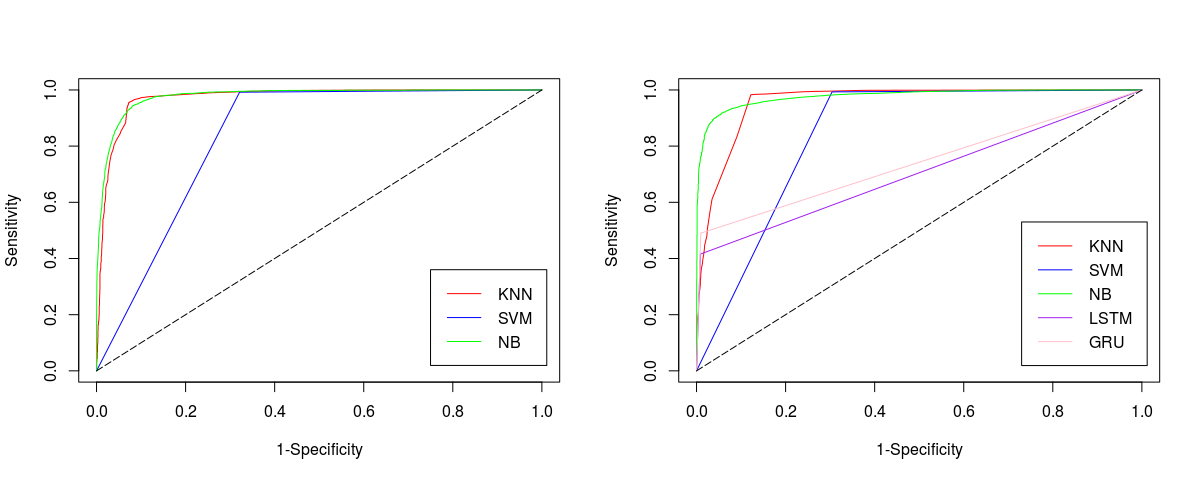
\includegraphics[width=1.0\textwidth]{figures/roc-curves.png}
    \caption{\textbf{Receiver operating characteristic curves showing the performance of binary classifiers for the segmentation of e-coaching text when lexical features (left) and combination of lexical and other features (right) are used}.}
    \label{fig:roc-curves}
\end{figure}

In this paper, results are reported by each class to avoid confusion about the overall model performance. In addition, standard metrics: precision, recall, and F1-measure were used to eliminate doubt about the model performance because accuracy is misleading for imbalance dataset. AUC values are also outlined due to its effectiveness in measuring the quality of binary classifiers for imbalanced datasets\cite{hu2015kernelized}, which are demonstrated by the ROC curves in Figure~\ref{fig:roc-curves}. NB shows the highest AUC values, achieved 0.978 for both cases while provides lowest classification results. On the other hand, KNN and SVM exhibit 0.972 and 0.835 AUCs when only lexical features are used; and 0.959 and 0.844 AUCs when a combination of lexical, punctuation mark and topic model-based features are used. Finally, LSTM demonstrates lowest AUC values among all machine learning models, achieved 0.82 AUC while GRU achieves 4.15\% higher AUC than LSTM. The conclusion drawn from the ROC curves also confirmed the robustness and superiority of KNN model for the segmentation of clinical exchange.      

We observed the second highest performance of RNN, in particular, LSTM and GRU for the text segmentation. We believe that RNN will perform better if a large set of data is utilized. In this study, we employed 3,138 examples of boundary case which limit to achieve the best performance. We also observed that GRU performs better than LSTM which was observed in other previous study\cite{chung2014empirical}.

Although punctuation mark plays an important role in segmentation boundary detection, and large numbers of errors were encountered by the false positive of boundary identification. For example, a text block ``A1 A2 A3. B1 B2 B3. C1 C2 C3 C4.'' can be incorrectly segmented at position A3, B3, and C4 where a punctuation mark was encountered. Similarly, additional information is the common reason for the classified original segment into multiple segments. For instance, the above text block can also be incorrectly segmented at position B3 and C4 because third sentence (C) only supports the MI code confirmed by first two sentences (A and B). 

Our proposed approach is novel for the segmentation of e-coaching text because previous studies mainly focus on the segmentation of text into sections, headers, and sentences in other medical domain. However, this study segmented clinical exchange into groups of MI behaviors which will significantly reduce the amount of resource and time required to segment clinical exchange manually. Furthermore, these segmentation models could be integrated with auto coding classifiers to build a software package of automatic coding procedure of clinical exchange.

The limitation of this study is that e-coaching text is collected from a single medical institute; formatting, style, and email segment can be different in other settings. Therefore, there is a need to replicate the experiments with different data sets. As our future work, we plan to evaluate our approach on other datasets involves in discourse analysis. We also plan to use more relevant features to improve model performance. For example, part-of-speech tagging\cite{hasan2016feedback} and distance from the beginning and end of the current sentence might significantly enhance the classification performance. 
 
\section*{Conclusion}
Segmentation of e-coaching text is an integral part of developing an automated e-coaching intervention. Although several studies have done in clinical interventions, they are limited by the qualitative coding of clinical interactions. In addition, previous studies in the medical domain mainly segmented clinical text into sections and sentences, none of them are used for the segmentation of text into groups of MI behaviors in the setting of discourse analysis with email under the principle of motivational interviews. In this paper, we compared the performance of machine learning models for the task of segmentation of e-coaching text. We found out that k-nearest neighbor provides the best performance for the segmentation of text in terms of all performance metrics. Manual segmentation of e-coaching data is very resource-intensive and time-consuming task, which can significantly decrease the time and effort required to develop an effective behavioral intervention. Our proposed methods can help to identify individual text segments, which can be annotated directly with a classification model. This approach will also help for developing fully automated e-coaching and accelerate the pace of identifying effective communication strategies.

\section*{Acknowledgments}
This study was supported by a grant from the National Institutes of Health, NIDDK R21DK108071, Carcone and Kotov, MPIs. We would like to thank research staff and student assistants in the Department of Family Medicine and Public Health Sciences at Wayne State University School of Medicine for their help in preparing the training dataset. 

\bibliographystyle{vancouver}
\bibliography{manuscript}

\end{document}
